% snsm_rsl.tex - Taylor & Francis Interact layout + Chicago author-date reference style
% Prepared from interactcadsample.tex (v1.04, May 2023) document conventions.
% Remote Sensing Letters submission draft (Research Letter, max 12 pages incl. tables and references).
% All table values and \snsm... macros are generated by experiments/make_paper_tables.py
% from experiments/results/*.csv -- regenerate, never edit numbers by hand.
%
% Template notes (do not edit this header when adding content):
% - interact.cls already loads amsmath, amssymb, amsfonts, amsthm, booktabs, epsfig,
%   graphicx and rotating; do not load geometry or use class options 10pt/11pt/12pt,
%   onecolumn/twocolumn, oneside/twoside, leqno/titlepage.
% - Citations are Chicago author-date via natbib (T&F tfcad.bst): \citep{key};
%   see \bibpunct below and interactcadsample.tex, Section "References".
% - Table captions appear ABOVE the table via \tbl{caption}{body}; tables' \label
%   goes just before \end{table}; figures' \label goes just after \caption.
% - Do not use [htb] float specifiers; rely on default placement ([p] or endfloat
%   only if the journal requires figures/tables separated from text).
\documentclass[]{interact}

\usepackage{tikz}
\usetikzlibrary{positioning,arrows.meta}
\usepackage{url}

\usepackage{natbib}% Citation support using natbib.sty
\bibpunct[, ]{(}{)}{;}{a}{}{,}% Citation support using natbib.sty
\renewcommand\bibfont{\fontsize{10}{12}\selectfont}% Bibliography support using natbib.sty

\newcommand{\ntrainIP}{505}
\newcommand{\ntestIP}{9{,}744}
\newcommand{\ntrainKSC}{256}
\newcommand{\ntestKSC}{4{,}955}
\newcommand{\ntrainPU}{2{,}135}
\newcommand{\ntestPU}{40{,}641}
\newcommand{\ntrainBW}{156}
\newcommand{\ntestBW}{3{,}092}
\newcommand{\ntrainIPstd}{695}
\newcommand{\ntestIPstd}{9{,}671}
\newcommand{\ntrainIPcnt}{695}
\newcommand{\ntestIPcnt}{9{,}554}
\newcommand{\djtestPU}{33{,}847--36{,}453}
\newcommand{\djclassesPU}{9}
\newcommand{\djtestKSC}{3{,}077--3{,}513}
\newcommand{\djclassesKSC}{11}
\newcommand{\dropPU}{32.0}
\newcommand{\spreadDJPU}{1.80}
\newcommand{\dropKSC}{34.3}
\newcommand{\spreadDJKSC}{4.44}
\newcommand{\spreadIPRand}{3.84}
\newcommand{\spreadIPSmall}{0.60}
\newcommand{\spreadIPCnt}{0.14}
\newcommand{\spreadIPStd}{0.35}
\newcommand{\nsigIPrand}{5}
\newcommand{\ciwIPrand}{2.2}
\newcommand{\nsigIPcnt}{0}
\newcommand{\ciwIPcnt}{0.3}
\newcommand{\nsigIPstd}{1}
\newcommand{\ciwIPstd}{0.4}
\newcommand{\nsigPUdj}{0}
\newcommand{\ciwPUdj}{4.0}
\newcommand{\nsigKSCdj}{3}
\newcommand{\ciwKSCdj}{3.9}
\newcommand{\nsigIPsmall}{7}
\newcommand{\ciwIPsmall}{0.6}
\newcommand{\nsigPUscarce}{2}
\newcommand{\ciwPUscarce}{1.7}
\newcommand{\nsigKSCscarce}{0}
\newcommand{\ciwKSCscarce}{2.0}
\newcommand{\spreadSCIPfive}{3.84}
\newcommand{\spreadSCIPsmall}{0.60}
\newcommand{\spreadSCPUfive}{0.31}
\newcommand{\spreadSCPUscarce}{1.59}
\newcommand{\spreadSCKSCfive}{0.32}
\newcommand{\spreadSCKSCscarce}{1.65}
\newcommand{\ipRandGain}{1.75--3.84}
\newcommand{\ipRandGainShort}{1.8--3.8}
\newcommand{\ipRandGainInt}{2--4}
\newcommand{\randOtherSpread}{0.32}
\newcommand{\kscFixedRange}{99.2--99.5}
\newcommand{\pcGpmDisp}{80.0--84.4}
\newcommand{\pcGpmRest}{62.7--78.5}
\newcommand{\pcOatsDisp}{66.3--77.2}
\newcommand{\pcOatsRest}{36.8--56.1}
\newcommand{\pcAlfalfaSpread}{3.3}
\newcommand{\cntCImax}{0.3}
\newcommand{\stdEcaDiff}{0.33}
\newcommand{\smallGain}{0.30--0.60}
\newcommand{\spreadSCIPsmallShort}{0.6}
\newcommand{\dropScarcePU}{15}
\newcommand{\dropScarceKSC}{7}
\newcommand{\djOAPU}{55--57}
\newcommand{\djOAKSC}{74--77}
\newcommand{\dropRange}{32--34}
\newcommand{\djStdRange}{4.4--7.4}
\newcommand{\ablMeanDrop}{1.16}
\newcommand{\paramsEca}{6}
\newcommand{\paramsSe}{4{,}256}
\newcommand{\paramsSnsm}{260}
\newcommand{\latencyRatio}{3.7}
\newcommand{\trainRatio}{1.7}
\newcommand{\margin}{1}
\newcommand{\seedSdIP}{2.2}
\newcommand{\bhSig}{16}
\newcommand{\bhTotal}{56}
\newcommand{\holmSig}{18}
\newcommand{\nSettings}{8}
\newcommand{\neqPUscarce}{1}
\newcommand{\neqKSCscarce}{2}
\newcommand{\ipRandOAspread}{0.17}
\newcommand{\nseedsIP}{15}


\begin{document}

\articletype{RESEARCH LETTER}

\title{Spectral-neighbourhood self-modulation for lightweight hyperspectral image classification with scarce labels}

\author{
\name{Swati Hira\textsuperscript{a}\thanks{CONTACT Swati Hira. Email: shira@iiitn.ac.in}, Devguru Tiwari\textsuperscript{a}, Pratibha Kokardekar\textsuperscript{b} and S.~R. Sathe\textsuperscript{c}}
\affil{\textsuperscript{a}Department of Computer Science and Engineering, IIIT Nagpur, Nagpur, India; \textsuperscript{b}RBU, Nagpur, India; \textsuperscript{c}VNIT, Nagpur, India}
}

\maketitle

\begin{abstract}
Channel-attention blocks in lightweight networks for hyperspectral image classification with scarce labels usually gate channels from globally pooled means and ignore how other statistics vary across neighbouring feature channels. We propose spectral-neighbourhood self-modulation (SNSM), a residual-block modulation in which each channel's scale and shift are predicted by a small one-dimensional convolution over per-channel mean, variance and cross-channel gradient. SNSM adds about 130 parameters per block and is initialised as the identity. Under one fixed protocol (five seeds, 100 epochs, no validation-based model selection), SNSM reaches \snsmIndianPinesAA\% average accuracy (AA) on Indian Pines with 5\% labelled pixels, the highest among SE, ECA, CBAM, HybridSN and SSFTT baselines, and it also leads there with 1\% and 10\% labels. Paired ablations attribute the gain mainly to the variance descriptor and the identity initialisation; the gradient descriptor and the additive shift each change AA by less than one point. The gains are in AA rather than overall accuracy and concentrate in small classes. On Kennedy Space Center (KSC), Pavia University and Botswana all CNN variants exceed 98.6\% AA. We also show that KSC stores small negative values as large unsigned integers; correcting this raises the CNN variants from 77--92\% to over 99\% AA.
\end{abstract}

\begin{keywords}
Hyperspectral image classification; channel attention; feature modulation; few labels; lightweight CNN
\end{keywords}

\section{Introduction}
Hyperspectral images record hundreds of contiguous bands. This makes pixel-level land-cover classification possible, but when labelled samples are few it exposes classifiers to the Hughes phenomenon \citep{hughes1968mean,bioucas2013analysis}. Kernel classifiers such as support vector machines \citep{camps2005kernel,melgani2004classification} and spectral--spatial methods \citep{fauvel2013advances,ghamisi2017advanced} were the standard before deep learning. Deep models now dominate \citep{li2019overview,audebert2019review}. Stacked autoencoders \citep{chen2014deep}, recurrent networks \citep{mou2017rnn} and graph convolutional networks \citep{hong2021gcn} have all been applied. Convolutional neural networks (CNNs) that operate on spatial--spectral patches are still the usual lightweight choice \citep{hu2015deep,makantasis2015deep,chen2016deep,li2017spectral,zhong2018ssrn,roy2020hybridsn}. Transformers bring global context, but at a higher training cost \citep{hong2022spectralformer,sun2022ssftt}.

Channel attention is a cheap way to make a CNN input-dependent. Squeeze-and-excitation (SE) \citep{hu2018squeeze} predicts one scale per channel from globally pooled features through two fully connected (FC) layers. CBAM adds spatial attention \citep{woo2018cbam}; ECA replaces the FC layers by a one-dimensional convolution over the pooled channel vector \citep{wang2020eca}; SRM pools channel means and standard deviations \citep{lee2019srm}; GCT normalises per-channel statistics and gates them with $1+\tanh(\cdot)$ from an identity start \citep{yang2020gct}; FcaNet replaces average pooling by several frequency components \citep{qin2021fcanet}. All of these predict a scale only. FiLM adds a shift but takes its conditioning from an external input \citep{perez2018film}. Hyperspectral networks have adopted these blocks widely, usually combining SE-style channel gates with spatial attention \citep{mei2019attention,haut2019attention,li2020dbda,zhu2021rssan,roy2021a2s2k}. With very few labelled pixels, FC gating has many parameters relative to the training set. Global means alone also discard how the response is spread within the patch.

We study a modulation that is (i) local across channels, (ii) driven by several per-channel statistics rather than the mean only, and (iii) identity at initialisation. Our contributions are:
\begin{itemize}
\item SNSM, a residual-block modulation whose scale and shift come from a dilated one-dimensional convolution over normalised channel means, variances and cross-channel gradients (Section~\ref{sec:method});
\item a single-protocol comparison on four scenes (plus two near-saturated scenes for SNSM alone), with label budgets of 1\%, 5\% and 10\% on IP and KSC, in which every model, including HybridSN and SSFTT, is trained on the same splits, inputs and schedule with no validation-based checkpoint selection (Section~\ref{sec:setup});
\item a correction of the KSC data encoding, without which the CNN variants appear 7--22 AA points less accurate on KSC (Section~\ref{sec:setup});
\item paired same-seed ablations that separate the effects of the descriptors, the identity initialisation and the additive shift (Section~\ref{sec:results}).
\end{itemize}

\section{Method}\label{sec:method}
\subsection{Input features}
Each band of the raw cube is smoothed with a $5\times5$ adaptive Wiener filter. Principal component analysis (PCA) \citep{jolliffe2016pca} then reduces the spectrum to 30 components; it is fitted without labels on all pixels of the scene. A one-level db4 discrete wavelet transform \citep{mallat1989theory,daubechies1992ten} is applied to each component. Its approximation sub-band, resized bilinearly to the image size, is concatenated with the components, giving $B=60$ features per pixel. Each labelled pixel is represented by the $15\times15\times B$ patch centred on it (zero padding at the image border).

\subsection{Backbone}
A $3\times3$ convolution maps the $B$ input features to $C=64$ channels (batch normalisation \citep{ioffe2015batch}, ReLU). Two residual blocks \citep{he2016deep} follow, each computing
\begin{equation}
\mathbf{h}=\mathrm{ReLU}(\mathrm{BN}(\mathrm{Conv}_{3\times3}(\mathbf{x}))),\qquad
\mathbf{y}=\mathrm{ReLU}\big(\mathrm{BN}(\mathrm{Conv}_{3\times3}(\mathcal{M}(\mathbf{h})))+\mathbf{x}\big),
\end{equation}
where $\mathcal{M}$ is the modulation under study ($\mathcal{M}=$ identity for the plain CNN). Global average pooling, dropout (0.4) \citep{srivastava2014dropout} and a linear layer produce the class scores.

\subsection{Spectral-neighbourhood self-modulation}
For $\mathbf{h}\in\mathbb{R}^{C\times H\times W}$, SNSM first computes three descriptors for every channel $c$: the spatial mean $\mu_c$, the spatial variance $v_c$, and the cross-channel gradient $g_c=(\mu_{c+1}-\mu_{c-1})/2$ (one-sided differences at the first and last channel). Each descriptor vector is standardised across channels, $\tilde{s}=(s-\bar{s})/(\sigma_s+\epsilon)$, and the three are stacked into $\mathbf{S}\in\mathbb{R}^{3\times C}$. Two one-dimensional convolutions along the channel axis give
\begin{equation}
\mathbf{Z}=\mathrm{Conv1D}^{(2)}_{k=3}\big(\mathrm{ReLU}(\mathrm{Conv1D}^{(1)}_{k=3,\,d=2}(\mathbf{S}))\big)\in\mathbb{R}^{2\times C},
\end{equation}
with 8 hidden channels, dilation $d=2$ in the first layer and replicate padding. The modulation is
\begin{equation}
\gamma_c=1+\tfrac12\tanh(Z_{1,c}),\qquad \beta_c=Z_{2,c},\qquad \mathcal{M}(\mathbf{h})_c=\gamma_c\,\mathbf{h}_c+\beta_c .
\end{equation}
The weights and bias of $\mathrm{Conv1D}^{(2)}$ are initialised to zero, so every block starts as the plain residual block and $\gamma_c\in[0.5,1.5]$ thereafter. The modulation adds 130 parameters per block, against 2{,}128 for SE gating with reduction to 16 units. Each channel's parameters depend on a window of neighbouring channels (receptive field of seven channels), as in ECA \citep{wang2020eca}. Unlike ECA, SNSM uses dispersion and gradient descriptors in addition to the mean, outputs a shift as well as a scale, and starts from the identity. The bounded gate and identity start resemble GCT \citep{yang2020gct}, and SRM also uses channel dispersion \citep{lee2019srm}. SNSM differs from both in filtering several descriptors jointly across neighbouring channels and in predicting a shift. The SNSM ($\gamma$) variant drops the shift output. Figure~\ref{fig:block} shows the data flow.

\begin{figure}[t]
\centering
\resizebox{\textwidth}{!}{% SNSM modulation inside a residual block (TikZ; included from snsm_rsl.tex).
\begin{tikzpicture}[
  font=\footnotesize, node distance=4mm and 5mm,
  box/.style={draw=black!70, rounded corners=2pt, align=center, minimum height=11mm, inner sep=3pt},
  op/.style={box, fill=blue!8},
  arr/.style={-{Stealth[length=2mm]}, black!70}]
\node[box] (h) {$\mathbf{h}\in\mathbb{R}^{C\times H\times W}$\\[1pt]\scriptsize Conv--BN--ReLU};
\node[op, right=of h] (d) {Per-channel descriptors\\[1pt]$\mu_c,\; v_c,\; g_c$\\[1pt]\scriptsize standardised over $c$};
\node[op, right=14mm of d] (c1) {Conv1D $3\!\to\!8$\\[1pt]\scriptsize $k{=}3$, $d{=}2$, ReLU};
\node[op, right=of c1] (c2) {Conv1D $8\!\to\!2$\\[1pt]\scriptsize $k{=}3$, zero init};
\node[op, below=7mm of c2] (gb) {$\gamma_c=1+\tfrac12\tanh Z_{1,c}$\\[1pt]$\beta_c=Z_{2,c}$};
\node[box, left=of gb, fill=blue!18] (m) {$\gamma_c\,\mathbf{h}_c+\beta_c$};
\node[box, below=5mm of m] (out) {Conv--BN, $+\mathbf{x}$, ReLU};
\draw[arr] (h) -- (d);
\draw[arr] (d) -- node[above]{\scriptsize $\mathbf{S}\in\mathbb{R}^{3\times C}$} (c1);
\draw[arr] (c1) -- (c2);
\draw[arr] (c2) -- node[right]{\scriptsize $\mathbf{Z}\in\mathbb{R}^{2\times C}$} (gb);
\draw[arr] (gb) -- (m);
\draw[arr] (h.south) |- ([yshift=2mm]m.west) ;
\draw[arr] (m) -- (out);
\end{tikzpicture}
}
\caption{SNSM inside a residual block. Per-channel descriptors of the feature map $\mathbf{h}$ are filtered along the channel axis by two one-dimensional convolutions, whose output sets a bounded scale $\gamma_c$ and a shift $\beta_c$ for each channel. The second convolution starts at zero, so the block is initially the identity.}
\label{fig:block}
\end{figure}

\section{Experimental setup}\label{sec:setup}
\textbf{Data.} We use Indian Pines (IP), Pavia University (PU), Kennedy Space Center (KSC), Botswana (BW), Salinas and WHU-Hi HanChuan \citep{baumgardner2015indian,gamba2004pavia,gic2020hyperspectral,zhong2020whu}. For each class, 5\% of the labelled pixels (at least one) are drawn at random for training; the remaining labelled pixels are used for testing. For Salinas and WHU-Hi, a random subset of 50{,}000 test pixels is used. This gives \ntrainIndianPines/\ntestIndianPines\ (IP), \ntrainKSC/\ntestKSC\ (KSC), \ntrainPaviaU/\ntestPaviaU\ (PU) and \ntrainBotswana/\ntestBotswana\ (BW) training/test pixels (Table~\ref{tab:data}). At 5\%, three IP classes (Alfalfa, Grass-pasture-mowed and Oats) have only one or two training pixels. KSC is distributed as unsigned 16-bit integers, but it contains small negative values ($-27$ to $-1$) that are stored in two's complement and are therefore read as 65{,}509--65{,}535; about 5\% of its pixels contain at least one such value. We read KSC as signed 16-bit integers. Without this correction, the wrapped values dominate the PCA and the CNN variants reach only 77--92\% AA on KSC at 5\% labels instead of 99.2--99.5\%.

\begin{table}[t]
\tbl{Benchmark scenes and the 5\% splits used (seed 42; split sizes are the same for every seed).}
{\resizebox{\textwidth}{!}{\begin{tabular}{llrrrrrr}
\toprule
Scene & Sensor & Size (pixels) & Bands & GSD (m) & Classes & Labelled & Train/test (random) \\
\midrule
Indian Pines (IP) & AVIRIS & $145\times145$ & 200 & 20 & 16 & 10,249 & 505/9,744 \\
Pavia University (PU) & ROSIS & $610\times340$ & 103 & 1.3 & 9 & 42,776 & 2,135/40,641 \\
Kennedy Space Center (KSC) & AVIRIS & $512\times614$ & 176 & 18 & 13 & 5,211 & 256/4,955 \\
Botswana (BW) & Hyperion & $1476\times256$ & 145 & 30 & 14 & 3,248 & 156/3,092 \\
\bottomrule
\end{tabular}
}}
\label{tab:data}
\end{table}

\textbf{Models.} On IP, KSC, PU and BW we compare seven modulation variants on the same backbone, plus HybridSN \citep{roy2020hybridsn} in its original layer configuration. The variants are: plain CNN; SE ($\gamma$) \citep{hu2018squeeze}; ECA ($\gamma$) \citep{wang2020eca}, with kernel size 3 as given by its adaptive rule for 64 channels; CBAM \citep{woo2018cbam}, with channel reduction 16 and a $7\times7$ spatial gate; FC ($\gamma{+}\beta$), i.e.\ SE-style FC layers predicting a sigmoid scale and a linear shift; SNSM ($\gamma$); and SNSM ($\gamma{+}\beta$). SSFTT \citep{sun2022ssftt} (four tokens, one transformer layer with eight heads) is reimplemented and run on IP and KSC only. Salinas and WHU-Hi are near saturation and are run with SNSM only.

\textbf{Protocol.} Every model sees the same 60-feature patches and the same splits for a given seed. Training uses cross-entropy, AdamW \citep{loshchilov2019decoupled} (learning rate $10^{-3}$, weight decay $10^{-4}$), a step decay (factor 0.5 every 40 epochs), batch size 64 and exactly 100 epochs, with no data augmentation and no early stopping. The final-epoch model is evaluated once. No validation or test data are used for model selection. Each configuration is repeated with seeds 42--46, and we report mean $\pm$ sample standard deviation. Runs used PyTorch \citep{paszke2019pytorch} on an NVIDIA Tesla T4. Baselines are therefore trained under our protocol and inputs rather than their original settings, so their accuracies are not directly comparable to published values.

\section{Results}\label{sec:results}
\begin{table}[t]
\tbl{OA and AA (\%, mean $\pm$ std over five seeds) at 5\% labelled pixels. Best mean per column in bold.}
{\resizebox{\textwidth}{!}{\begin{tabular}{lcccccccc}
\toprule
Method & \multicolumn{2}{c}{IP} & \multicolumn{2}{c}{KSC} & \multicolumn{2}{c}{PU} & \multicolumn{2}{c}{BW} \\
 & OA & AA & OA & AA & OA & AA & OA & AA \\
\midrule
Plain CNN & 96.28$\pm$0.79 & 89.49$\pm$2.44 & 99.65$\pm$0.34 & 99.51$\pm$0.36 & \textbf{99.59$\pm$0.07} & 99.01$\pm$0.16 & 99.09$\pm$0.55 & 98.87$\pm$0.90 \\
SE ($\gamma$) & \textbf{96.34$\pm$0.62} & 90.04$\pm$2.18 & 99.61$\pm$0.28 & 99.43$\pm$0.38 & 99.53$\pm$0.19 & 98.80$\pm$0.56 & 98.95$\pm$0.82 & 98.76$\pm$1.07 \\
ECA ($\gamma$) & 96.28$\pm$0.68 & 90.87$\pm$2.53 & 99.61$\pm$0.47 & 99.40$\pm$0.66 & 99.58$\pm$0.10 & 99.00$\pm$0.20 & \textbf{99.13$\pm$0.76} & \textbf{98.90$\pm$1.08} \\
CBAM & 96.19$\pm$0.60 & 91.58$\pm$1.49 & 99.54$\pm$0.56 & 99.23$\pm$0.83 & 99.58$\pm$0.06 & \textbf{99.11$\pm$0.18} & 98.99$\pm$0.87 & 98.78$\pm$1.20 \\
GCT & 96.28$\pm$0.80 & 90.07$\pm$2.34 & \textbf{99.69$\pm$0.26} & \textbf{99.55$\pm$0.28} & 99.58$\pm$0.08 & 98.99$\pm$0.18 & 99.11$\pm$0.56 & 98.88$\pm$0.91 \\
SRM & 96.20$\pm$0.71 & 93.04$\pm$2.14 & 99.69$\pm$0.36 & 99.51$\pm$0.49 & 99.55$\pm$0.07 & 98.92$\pm$0.17 & 98.87$\pm$0.63 & 98.67$\pm$0.97 \\
SNSM ($\gamma$) & 96.17$\pm$0.73 & 92.89$\pm$2.00 & 99.69$\pm$0.26 & 99.50$\pm$0.39 & 99.49$\pm$0.05 & 98.91$\pm$0.16 & 99.10$\pm$0.62 & 98.89$\pm$0.96 \\
SNSM ($\gamma{+}\beta$) & 96.27$\pm$0.67 & \textbf{93.33$\pm$1.68} & 99.63$\pm$0.55 & 99.45$\pm$0.73 & 99.47$\pm$0.05 & 98.93$\pm$0.16 & 99.04$\pm$0.69 & 98.85$\pm$1.03 \\
\bottomrule
\end{tabular}
}}
\label{tab:main}
\end{table}

\textbf{Accuracy.} Table~\ref{tab:main} gives the main comparison. On IP, SNSM ($\gamma{+}\beta$) has the highest AA; SSFTT and CBAM have higher OA but lower AA. On KSC, PU and BW the AA of the seven CNN variants lies within about 0.3 points, so modulation brings no measurable benefit on these scenes. HybridSN trained under our protocol is less accurate and less stable; on one BW seed it did not converge (\hybridBWmin\% OA). SNSM reaches \snsmSalinasOA\% OA on Salinas and \snsmWHUOA\% OA on WHU-Hi. Figure~\ref{fig:aa} shows the AA spread across seeds on IP and KSC.

\begin{figure}[t]
\centering
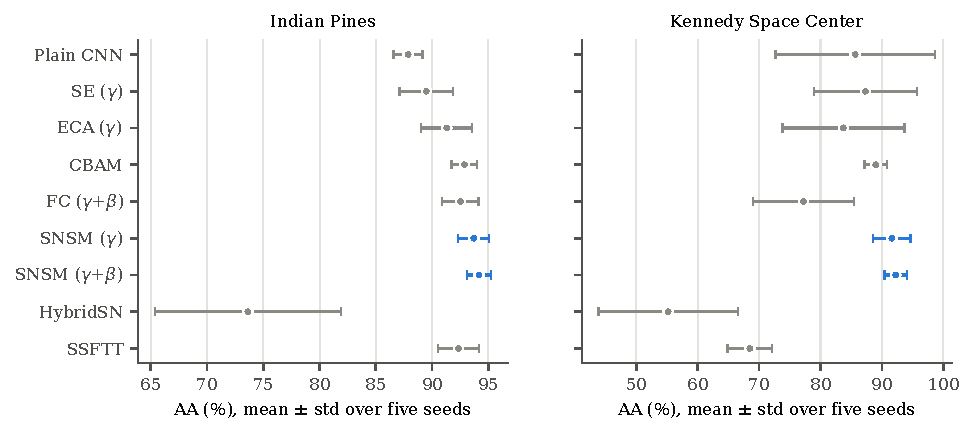
\includegraphics[width=\textwidth]{figures/aa_by_model.pdf}
\caption{AA (mean $\pm$ standard deviation over five seeds) on Indian Pines and Kennedy Space Center. SNSM variants in blue. On KSC all CNN variants lie above 99\%.}
\label{fig:aa}
\end{figure}

\begin{table}[t]
\tbl{Paired same-seed differences in AA (percentage points): mean over five seeds and number of seeds with a positive difference.}
{\begin{tabular}{lccccc}
\toprule
SNSM ($\gamma{+}\beta$) $-$ & IP random 5\% & IP random 50/15 & IP standard & PU disjoint & KSC disjoint \\
\midrule
Plain CNN & +3.84$^{*}$ [+2.6, +5.1] & -0.01 [-0.2, +0.2] & +0.24 [+0.1, +0.4] & +0.31 [-1.6, +2.2] & +3.46$^{*}$ [+1.7, +5.1] \\
SE ($\gamma$) & +3.29$^{*}$ [+2.4, +4.3] & -0.08 [-0.2, +0.0] & +0.23 [+0.1, +0.4] & -0.47 [-2.5, +1.4] & -0.19 [-2.1, +1.6] \\
ECA ($\gamma$) & +2.45$^{*}$ [+1.1, +3.9] & +0.04 [-0.1, +0.2] & +0.33$^{*}$ [+0.2, +0.5] & -0.39 [-2.2, +1.4] & +1.86 [+0.6, +3.3] \\
CBAM & +1.75$^{*}$ [+1.0, +2.5] & +0.05 [-0.1, +0.2] & +0.04 [-0.1, +0.2] & +1.03 [-0.6, +2.4] & +0.91 [-0.7, +2.4] \\
GCT & +3.26$^{*}$ [+2.2, +4.4] & +0.01 [-0.2, +0.2] & +0.25 [+0.1, +0.4] & +0.92 [-0.8, +2.5] & +3.51$^{*}$ [+1.8, +5.2] \\
SRM & +0.29 [-0.6, +1.3] & +0.07 [-0.1, +0.2] & -0.02 [-0.2, +0.1] & +1.33 [-0.3, +2.7] & +4.25$^{*}$ [+2.0, +6.6] \\
SNSM ($\gamma$) & +0.44 [-0.2, +1.1] & +0.06 [-0.1, +0.3] & +0.12 [-0.1, +0.3] & +0.03 [-1.7, +1.8] & +1.40 [-0.7, +3.6] \\
\bottomrule
\end{tabular}
}
\label{tab:paired}
\end{table}

\textbf{Where the gain comes from.} Table~\ref{tab:paired} and Figure~\ref{fig:paired} pair runs that share a seed and therefore a split. On IP, replacing SE gating by the SNSM descriptor network (both scale-only) raises AA in all five paired runs, by 4.22 points on average. ECA also gates each channel with a local convolution across channels, but it uses only the channel mean and has lower AA than SNSM ($\gamma$) on four of five seeds (by 2.41 points on average). Locality across channels alone therefore does not explain the gain; Table~\ref{tab:ablation} separates the descriptors and the initialisation. CBAM, which adds max pooling and a spatial gate to SE-style channel attention, has lower AA than SNSM ($\gamma{+}\beta$) on four of five seeds (by 1.30 points). Adding the shift to SNSM raises AA by only 0.46 points and helps on three of five seeds, so we do not claim a benefit from the shift itself, whereas adding a shift to FC gating raises AA by 3.02 points. On KSC, PU and BW every paired difference is below 0.25 points in magnitude.

\begin{figure}[t]
\centering
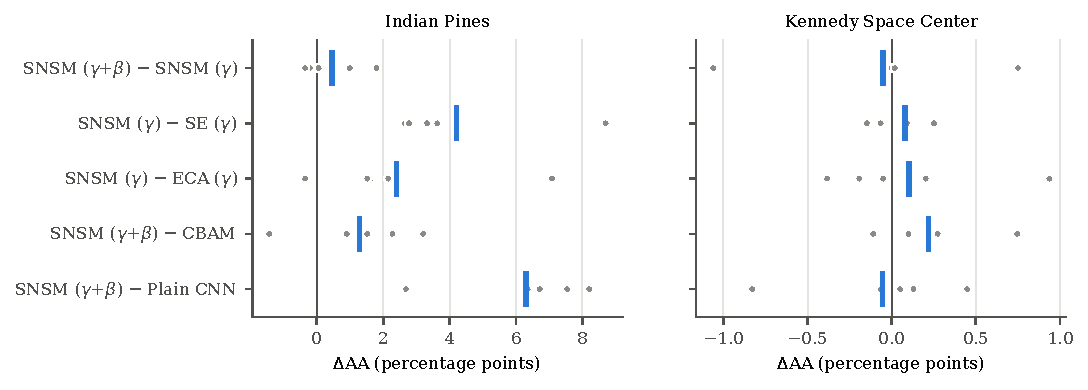
\includegraphics[width=\textwidth]{figures/paired_differences.pdf}
\caption{Paired same-seed differences in AA. Grey dots are the five seeds; the blue bar is their mean.}
\label{fig:paired}
\end{figure}

\textbf{Descriptors and initialisation.} Table~\ref{tab:ablation} removes descriptors from SNSM ($\gamma{+}\beta$) or drops its zero initialisation, again pairing runs by seed. On IP the variance descriptor carries most of the gain: with the mean alone, AA falls by 1.16 points, and adding the gradient to the mean recovers only 0.36 of them. Once the variance is present, the gradient lowers AA by 0.39 points. Without zero initialisation, AA is lower on all five seeds, by 1.49 points. On KSC, where all variants exceed 99\% AA, no ablation changes AA by more than 0.4 points.

\begin{table}[t]
\tbl{Descriptor and initialisation ablation of SNSM ($\gamma{+}\beta$) at 5\% labelled pixels. AA in \% (mean $\pm$ std over five seeds); $\Delta$AA is the paired difference from the full model and wins counts seeds on which the variant is better.}
{\resizebox{\textwidth}{!}{\begin{tabular}{lcccc}
\toprule
Descriptors & \multicolumn{2}{c}{IP} & \multicolumn{2}{c}{KSC} \\
 & AA & $\Delta$AA (wins/5) & AA & $\Delta$AA (wins/5) \\
\midrule
mean, var, grad (SNSM) & 94.16$\pm$1.07 & -- & 92.25$\pm$1.84 & -- \\
mean & 93.01$\pm$0.72 & -1.16 (1/5) & 83.81$\pm$7.78 & -8.44 (0/5) \\
mean, var & 94.55$\pm$1.67 & +0.39 (4/5) & 91.33$\pm$2.43 & -0.92 (1/5) \\
mean, grad & 93.37$\pm$1.09 & -0.80 (1/5) & 82.35$\pm$8.54 & -9.90 (1/5) \\
mean, var, grad; default init. & 92.67$\pm$1.15 & -1.49 (0/5) & 90.34$\pm$1.27 & -1.91 (0/5) \\
\bottomrule
\end{tabular}
}}
\label{tab:ablation}
\end{table}

\textbf{Label budget.} Table~\ref{tab:budget} repeats the comparison with 1\% and 10\% of the labelled pixels per class on IP and KSC (98 and 48 training pixels at 1\%; 1{,}018 and 516 at 10\%). On IP, SNSM ($\gamma{+}\beta$) has the highest AA at all three budgets; at 1\% and 10\% its margin over the CNN baselines is 0.4--2.0 points. At 1\% on IP it also has the lowest OA of the CNN variants (82.77\% against 84.23--85.26\%), so its advantage is again in AA rather than OA. On KSC, SNSM is never best: at 1\% all CNN variants reach 86--87\% AA with a seed-to-seed spread of 4--6 points, and at 5\% and 10\% they all exceed 99\%.

\begin{table}[t]
\tbl{AA (\%, mean $\pm$ std over five seeds) with 1\%, 5\% and 10\% labelled pixels per class. The 5\% column repeats Table~\ref{tab:main}. Best mean per column in bold.}
{\resizebox{\textwidth}{!}{\begin{tabular}{lcccccc}
\toprule
Method & \multicolumn{3}{c}{IP} & \multicolumn{3}{c}{KSC} \\
 & 1\% & 5\% & 10\% & 1\% & 5\% & 10\% \\
\midrule
Plain CNN & 83.51$\pm$1.23 & 87.86$\pm$1.29 & 96.69$\pm$1.43 & 55.40$\pm$2.45 & 85.64$\pm$12.98 & 76.90$\pm$10.69 \\
SE ($\gamma$) & 84.01$\pm$1.66 & 89.49$\pm$2.39 & 96.42$\pm$2.04 & 56.05$\pm$5.00 & 87.32$\pm$8.36 & 78.84$\pm$12.82 \\
ECA ($\gamma$) & 84.66$\pm$1.20 & 91.30$\pm$2.26 & 96.79$\pm$1.42 & 54.76$\pm$3.84 & 83.72$\pm$9.93 & 77.85$\pm$8.42 \\
CBAM & 83.08$\pm$1.15 & 92.87$\pm$1.14 & 96.20$\pm$1.94 & 60.47$\pm$2.79 & 89.00$\pm$1.82 & \textbf{87.12$\pm$8.78} \\
SNSM ($\gamma{+}\beta$) & \textbf{85.04$\pm$0.76} & \textbf{94.16$\pm$1.07} & \textbf{97.70$\pm$0.66} & \textbf{61.83$\pm$4.57} & \textbf{92.25$\pm$1.84} & 85.44$\pm$14.47 \\
SSFTT & 80.68$\pm$1.51 & 92.35$\pm$1.81 & 96.73$\pm$1.06 & 54.03$\pm$5.02 & 68.50$\pm$3.65 & 60.18$\pm$9.86 \\
\bottomrule
\end{tabular}
}}
\label{tab:budget}
\end{table}

The AA gains on IP come from small classes (Table~\ref{tab:perclass}). Relative to the plain CNN, SNSM ($\gamma{+}\beta$) raises mean per-class accuracy on Oats (20 labelled pixels) from 21.1\% to 74.7\%, on Grass-pasture-mowed (28) from 63.0\% to 92.6\%, and on Stone-Steel-Towers (93) from 76.9\% to 92.4\%. Oats and Grass-pasture-mowed have one training pixel and 19 and 27 test pixels, so these two gains correspond to about ten and eight test pixels. AA on IP is therefore sensitive to a few pixels, whereas the OA of all seven CNN variants on IP lies within 0.6 points. Figure~\ref{fig:map} shows the resulting IP classification map for one seed.

\begin{table}[t]
\tbl{Per-class accuracy (\%, mean over five seeds) on Indian Pines; $n$ is the number of labelled pixels. Best value per row in bold.}
{\resizebox{\textwidth}{!}{\begin{tabular}{lrrrrrrrrr}
\toprule
Class & $n$ & Plain CNN & SE ($\gamma$) & ECA ($\gamma$) & CBAM & SNSM ($\gamma$) & SNSM ($\gamma{+}\beta$) & HybridSN & SSFTT \\
\midrule
Alfalfa & 46 & 92.7 & 90.9 & 90.5 & 92.7 & \textbf{94.5} & 89.1 & 29.1 & 81.8 \\
Corn-notill & 1428 & 96.3 & 95.8 & 96.7 & 96.5 & 96.6 & 95.8 & 88.1 & \textbf{97.3} \\
Corn-mintill & 830 & 93.9 & 94.0 & 93.6 & \textbf{95.0} & 93.7 & 94.2 & 82.2 & 94.4 \\
Corn & 237 & 90.9 & 92.1 & 92.8 & 94.3 & 93.8 & \textbf{96.5} & 61.8 & 90.6 \\
Grass-pasture & 483 & 97.1 & \textbf{97.2} & 96.5 & 96.8 & 96.7 & 96.9 & 82.3 & 96.3 \\
Grass-trees & 730 & 97.3 & 96.5 & 97.2 & 97.8 & 97.2 & 97.7 & 97.8 & \textbf{98.4} \\
Grass-pasture-mowed & 28 & 63.0 & 58.5 & 84.4 & 89.6 & 88.9 & \textbf{92.6} & 44.4 & \textbf{92.6} \\
Hay-windrowed & 478 & 99.3 & \textbf{99.6} & 99.6 & 99.6 & 99.4 & 99.6 & 96.3 & 99.5 \\
Oats & 20 & 21.1 & 44.2 & 43.2 & 58.9 & 70.5 & \textbf{74.7} & 27.4 & 60.0 \\
Soybean-notill & 972 & 92.3 & 93.7 & 92.3 & 93.3 & 93.2 & 92.7 & 84.5 & \textbf{94.2} \\
Soybean-mintill & 2455 & 97.3 & \textbf{97.9} & 97.2 & 97.1 & 96.7 & 97.2 & 94.4 & 97.4 \\
Soybean-clean & 593 & 93.1 & 92.8 & 92.4 & 93.8 & 91.8 & 91.2 & 73.8 & \textbf{94.5} \\
Wheat & 205 & 96.4 & 97.7 & 96.6 & 97.1 & 96.8 & 98.2 & 85.4 & \textbf{98.6} \\
Woods & 1265 & 99.5 & 99.6 & 99.6 & 99.5 & 99.4 & 99.2 & 96.8 & \textbf{99.8} \\
Bldg-Grass-Trees-Drives & 386 & \textbf{98.9} & 98.1 & 98.8 & 98.2 & 98.1 & 98.7 & 89.1 & 97.9 \\
Stone-Steel-Towers & 93 & 76.9 & 83.1 & 89.4 & 85.6 & 91.7 & \textbf{92.4} & 44.9 & 84.3 \\
\midrule
AA & & 87.9 & 89.5 & 91.3 & 92.9 & 93.7 & 94.2 & 73.6 & 92.4 \\
\bottomrule
\end{tabular}
}}
\label{tab:perclass}
\end{table}

\begin{figure}[t]
\centering
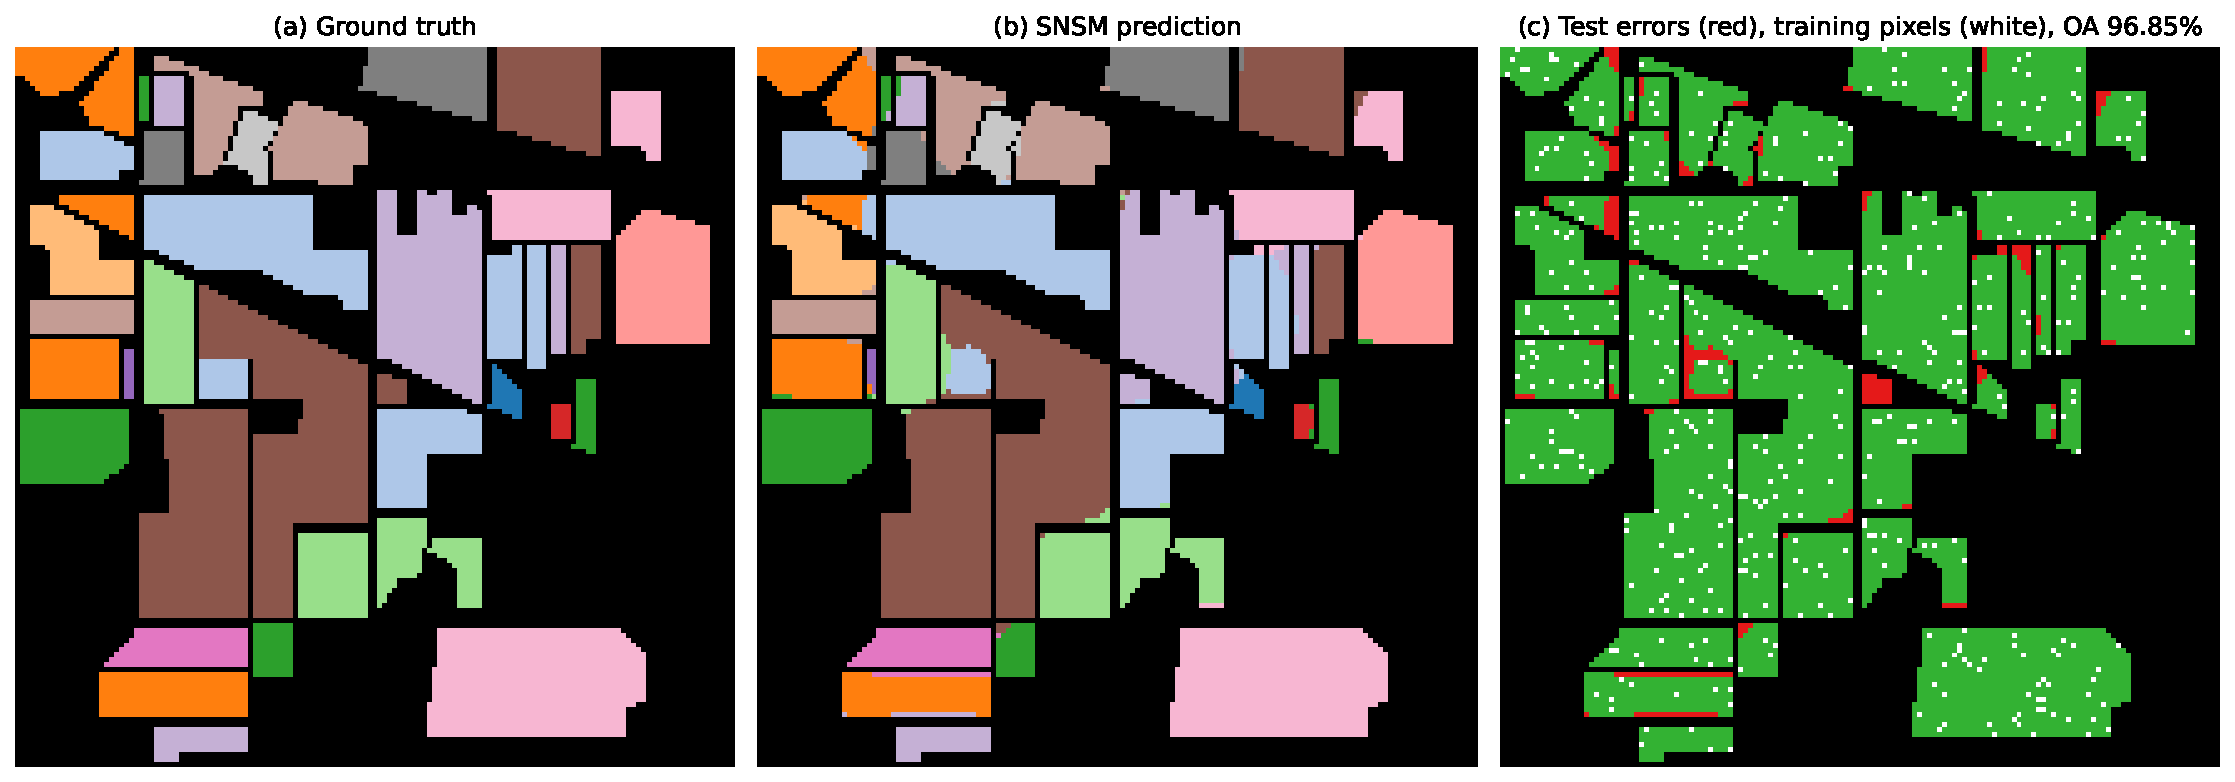
\includegraphics[width=\textwidth]{figures/classification_map_IndianPines.pdf}
\caption{Indian Pines, SNSM ($\gamma{+}\beta$), seed 42: (a) ground truth, (b) prediction for all labelled pixels, (c) test errors in red and training pixels in white.}
\label{fig:map}
\end{figure}

\begin{table}[t]
\tbl{Model size and cost for a $15\times15\times60$ IP patch. Training time is the mean per run (100 epochs).}
{\begin{tabular}{lrrrrr}
\toprule
Method & Params (M) & MMACs$^{a}$ & Latency (ms)$^{b}$ & Train IP (s) & Train PU (s) \\
\midrule
Plain CNN & 0.184 & 41.2 & 0.69 & 4.4 & 17.6 \\
SE ($\gamma$) & 0.188 & 41.2 & 1.17 & 4.6 & 19.3 \\
ECA ($\gamma$) & 0.184 & 41.2 & 0.98 & 5.2 & 19.8 \\
CBAM & 0.185 & 41.3 & 1.55 & 6.0 & 24.9 \\
FC ($\gamma{+}\beta$) & 0.190 & 41.2 & 1.31 & 4.7 & 19.8 \\
SNSM ($\gamma$) & 0.184 & 41.3 & 2.54 & 7.5 & 29.5 \\
SNSM ($\gamma{+}\beta$) & 0.184 & 41.3 & 2.54 & 7.6 & 30.2 \\
HybridSN & 1.743 & 137.4 & 0.71 & 26.2 & 115.3 \\
SSFTT & 0.291 & 34.9 & 1.25 & 7.6 & -- \\
\bottomrule
\end{tabular}
}
\tabnote{$^{a}$Multiply--accumulates of convolution and linear layers counted by \texttt{thop}; tensor operations such as attention products and descriptor statistics are not included. $^{b}$Batch size 1 on a Tesla T4.}
\label{tab:eff}
\end{table}

\textbf{Cost.} SNSM adds almost no parameters or multiply--accumulates to the plain CNN (Table~\ref{tab:eff}), but its descriptor computation consists of many small operations, so its batch-1 latency is about 3.7 times and its training time about 1.7 times that of the plain CNN. SNSM is lightweight in parameters and multiply--accumulates, not in wall-clock time. All CNN variants remain an order of magnitude smaller than HybridSN.

\section{Discussion and limitations}
Local cross-channel modulation helps on the scene with the smallest and most spectrally similar classes (IP), with fewer gating parameters than SE. On KSC, PU and BW a plain CNN is already near saturation at 5\% labels and the benefit disappears, and Salinas and WHU-Hi are near saturation for SNSM itself, so our evidence for a benefit rests on a single scene. Several limitations apply. Training and test pixels are drawn at random from the same scene, so overlapping patches share spatial context and accuracies are optimistic compared with spatially disjoint splits \citep{liang2017sampling,nalepa2019validating}. PCA is fitted on all pixels of each scene without labels. Five seeds give only an indication of variability, and the paired differences in Table~\ref{tab:paired} are not formal significance tests (with five pairs, a two-sided Wilcoxon signed-rank test cannot reach $p<0.05$). Baselines were not tuned to our protocol. HybridSN, and SSFTT on IP, are less accurate here than in their original papers, which used larger training sets and their own preprocessing and schedules, so our results describe only how they behave under this shared protocol. SNSM's hidden width, kernel size, dilation and scale bound were fixed in earlier exploratory runs on these scenes and were not tuned further. We report no sensitivity analysis for them. Finally, the channel order of learned feature maps has no physical wavelength meaning, so ``neighbourhood'' refers to adjacency of feature channels, which the first convolution is free to learn.

\section{Conclusion}
SNSM predicts per-channel scale and shift with a small convolution over neighbouring channels' mean, variance and gradient. Under a single strict protocol, with about 130 extra parameters per block, it gives the best average accuracy on Indian Pines at 1\%, 5\% and 10\% labels. On KSC (once its data encoding is corrected), Pavia University and Botswana, all CNN variants perform alike. Paired ablations attribute the improvement mainly to the variance descriptor and the identity initialisation, not to the gradient descriptor or the additive shift. The gains are in average rather than overall accuracy, and they cost a 3.7-fold increase in batch-1 latency.

\section*{Disclosure statement}
The authors report there are no competing interests to declare.

\section*{Funding}
No external funding was received for this research.

\section*{Data and code availability}
The datasets are publicly available \citep{gic2020hyperspectral,zhong2020whu}. Code, per-run results and the scripts that generate every table are available at \url{https://github.com/Devguru-codes/research_paper_code}.

\section*{Use of generative AI}
Generative AI (Claude, Anthropic) was used to assist with writing experiment code, checking references and editing the manuscript text. The authors reviewed and verified all code, results and text, and take full responsibility for the content.
\bibliographystyle{tfcad}
\bibliography{refs}

\end{document}
